\section{Multivariate Categorization}\label{sec:hmmBdt}

This section describes the division of the inclusive 3-lepton and 4-lepton categories into exclusive (``post-cut'') sub-categories.
The definition of the exclusive categories is based on a multivariate discriminant that is a function of several kinematic variables.
The discriminant is calculated using a \emph{boosted decision tree} (BDT) that is defined using the available information about signal and background kinematics from simulation.

\begin{figure}[h!]
\captionsetup[subfigure]{position=b}
\centering
\subfloat[][]{\label{fig:bdtTree}{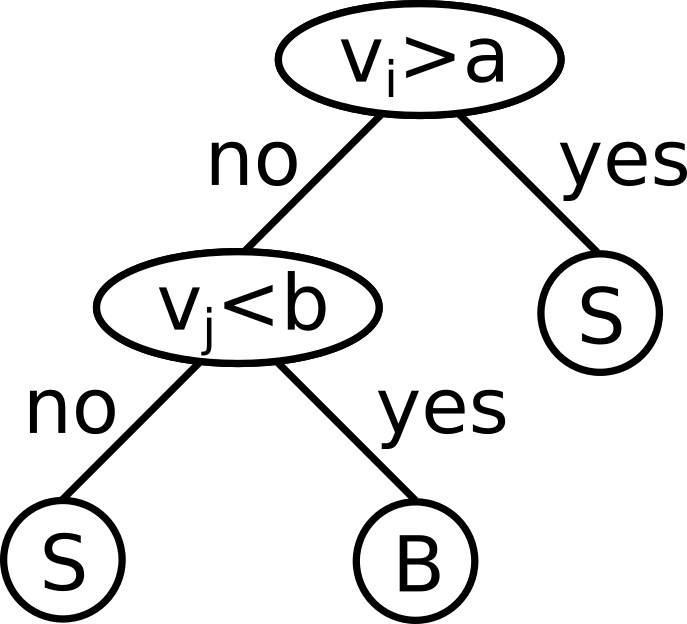
\includegraphics[width=0.25\textwidth]{figures/hmm/tree.png}}}
\subfloat[][]{{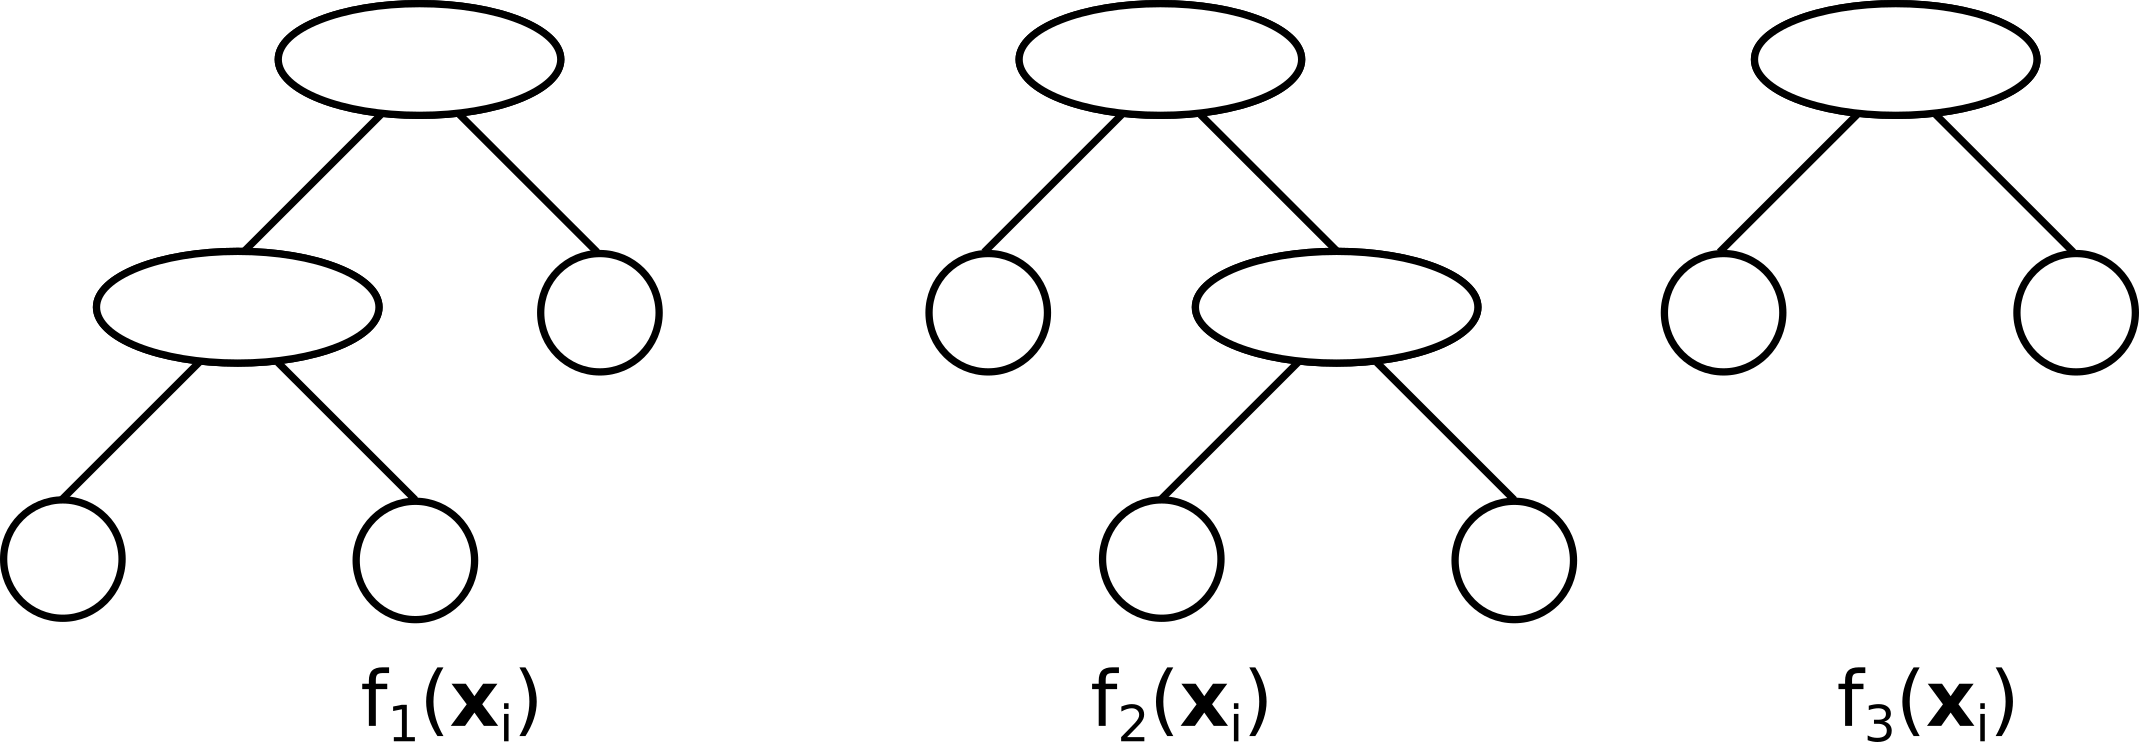
\includegraphics[width=0.75\textwidth]{figures/hmm/treeEnsamble.png}}}
\caption{Figure (a) schematizes an individual decision tree, where in boolean splits based on the value of variables $v$ result in a categorization of signal or data as output. In a CART, the output is replaced by a continuous weight encoding ``signal-like'' versus ``background-like''. Figure (b) schematizes an ensemble of trees with different topologies, each defining an output function.}
\label{fig:}
\end{figure}

At the basis of the BDT are trees and a dataset of $n$ entries and $m$ variables.
In its present usage, the classification is an example of supervised learning, so the entries $x_i$ $i\in[1,...,n]$ are labeled as either signal or background with $y_i$.
The elements of $x_i$ are variables $v_j$ $j\in[1,...,m]$.
A decision tree maps an entry of the dataset $x_i$ onto a discrete output space, such as a signal-vs-background likelihood.
Each node of the tree may represent a binary decision, or split, based on the variables of the entry.
Alternatively, the nodes with no children (leaves) may represent a decision, as illustrated in Figure \ref{fig:bdtTree}.
A generalization of a decision tree that assigns continuous weights to each leaf is a classification and regression tree (CART).
A tree can be \emph{trained} to map a set of input entries $x_i$ onto their corresponding labels $y_i$ by treating the distributions of input variables as PDFs and selecting splits (a, b, ...) that result in the highest output fidelity.
A single CART tends to struggle to represent the complexity of simulated physics datasets succinctly.
This performance can be augmented by an ensemble of CARTs labeled $k$, each with an output function $f_k(x_i)$ as illustrated in Figure \ref{fig:bdtTree}.
The output functions act as a \emph{model} of the provided dataset.
The sum of the CART output functions defines a new ensemble output function $f(x_i)=\hat{y}_i$, also called the discriminant score.

The strategy is to develop an ensemble whose output functions accurately predict the corresponding label $y_i$ for unseen events.
This is quantified by a regularized loss function,
\begin{equation}\begin{split}\label{eqn:lossFunc}
    \mathcal{L}(\phi)=\sum_i l(\hat{y}_i,y_i),
\end{split}\end{equation} 
where $l$ measures the difference between $\hat{y}_i$ and $y_i$.
A training process is defined to select trees, splits, and weights to minimize Equation \ref{eqn:lossFunc}.

\emph{Boosting} is a method to minimize such loss functions, provided it is differentiable, by ``boosting'' the capability of a CART.
Essentially it consists of iteratively expanding an ensemble of trees, with each addition addressing the miss-categorization of the previous ensemble.
One algorithm, AdaBoost, performs this task by iteratively reweighting poorly categorized entries to be more important to the following tree.
Another algorithm, Gradient Boosting, instead adds trees that are trained on the previous ensemble's poorly categorized entries.
A recent descendent of AdaBoost and Gradient Boosting is \xgb, which introduces a modified loss function,
\begin{equation}\begin{split}\label{eqn:lossFuncXgb}
    \mathcal{L}(\phi)=\sum_i l(\hat{y}_i,y_i)+\sum_k \Omega(f_k).
\end{split}\end{equation} 
In Equation \ref{eqn:lossFuncXgb}, $\Omega$ is a measure of the complexity a tree.
\xgb iteratively adds trees diminishing weights, shrinking their importance by a constant factor.
\xgb also introduces procedures to more quickly add and remove branches from trees while fitting the loss function.
These result in an output function that can be trained quickly.
The \xgb algorithm is used to construct the multivariate discriminant functions that are used in this analysis.
\cite{xgboost}

% Overtraining
It is a recurring theme in data analysis: to understand the underlying probability distributions that have produced a dataset, rather than of the dataset itself.
This applies to tasks such as training BDTs to discriminate signal from background, as well as fitting a functional form to data to model a background distribution. 
In both cases, the analytic model is interpreted as knowledge of these underlying distributions.
When solving an optimization problem such as those posed in Equations \ref{eqn:lossFunc} and \ref{eqn:lossFuncXgb}, the minimization algorithm has only the dataset at its disposal.
This can lead to \emph{over-training} or \emph{over-fitting}, where the optimization of the loss function tunes the discriminant to the features of a particular dataset rather than the features of the underlying distributions.
In general, this problem correlates with the complexity of the model.
It is combatted in part by penalizing the optimization by the complexity of the model, as is the case with the $\Omega$ function in Equation \ref{eqn:lossFuncXgb}.

From a physics analysis perspective, over-training may have two effects.
The first is to reduce the efficacy of the discriminant when applied to a new dataset.
This impacts the performance of the analysis, but it does not invalidate the results.
The real danger to the integrity of the analysis arises when the performance of the discriminant is inaccurately measured.
This second effect is illustrated in the following example.
Suppose a BDT is trained to identify signal events from a simulated dataset, and the same dataset is used to predict the number of signal events to expect in observed data.
A signal-rich category is defined based on the discriminant score for events.
In this case, simulated signal events tend to be over-represented in the category.
The BDT will identify simulated signal events with higher efficiency compared to signal in the data, leasing to an unconstrained uncertainty on the expected signal.
Unlike the first effect, this type of error invalidates the double use of the training simulation for further measurements.

\begin{figure}[h!]
\captionsetup[subfigure]{position=b}
\centering
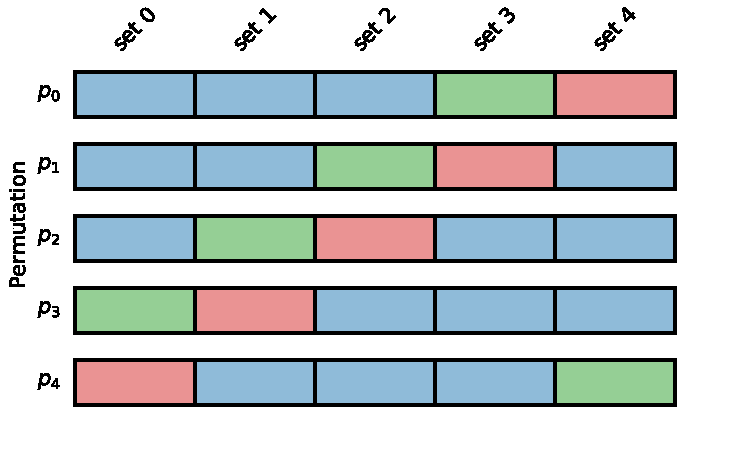
\includegraphics[width=0.75\textwidth]{figures/hmm/testTrainVal.pdf}
\caption{The top row, $p_0$, shows an schematization of a dataset divided into five subsets with $k$-fold split with $k=5$.
The blue boxes represent sets to be used for training, the green boxes for validation, the red boxes for testing.
Five permutations of these assignments, $p_i$, are shown for the same dataset.
In cross-validation, a separate MVA is fit to each permutation, such that each entry of the full dataset belongs to the testing set for a particular MVA.
}
\label{fig:testTrainVal}
\end{figure}

This problem is avoided by introducing the $k$-fold split of the available simulated datasets into $k>2$ subsets of equal multiplicity.
One subset is labeled as the ``testing'' set, and another is labeled as a ``validation'' set.
The remaining subsets are combined as a ``training'' set.
This is illustrated in the top of Figure \ref{fig:testTrainVal}.
The BDT is trained with the training set, and further predictions with respect to the simulation are performed with the testing set.
Since the testing set has not been exposed to the BDT during training, there is no chance of over-training of the discriminant scores in the testing set.
There remains the issue of selecting thresholds that define the signal-rich category to optimize, for example, the expected sensitivity.
This choice is subject to the same concerns about over-training as the selection of trees during the training phase. 
A third set, the validation set, is defined orthogonally to both the training and testing sets.
This set is used to study the convergence of the training process, check for over-training effects that may reduce sensitivity, and, most importantly, to choose the discriminant thresholds for further categorization.

The final consideration is to inefficiency that such a division of the simulation set entails.
Simulated events are computationally expensive to produce.
A \emph{cross-validation} scheme calls for the permutation of each of the $k$ subdivisions, such that each event appears once in a test set, available for further analysis.
This is shown in Figure \ref{fig:testTrainVal}.
A separate BDT is trained with the training set from each permutation.
This means that each event in the full dataset has one discriminant score from a BDT for which it is in the testing set, one for which it is in the validation set, and $k-2$ for which it was in the training set.
The scores from the BDT for which an event was in the testing and validation sets are the testing and validation scores, respectively.

\subsection{Configuration}
\label{sec:hmmBdtConfiguration}

% Training details
Separate classifiers are trained for 3-lepton and 4-lepton categories, but there are many similarities between these.
A 5-fold splitting of the available signal and background simulation is used.
It is important to note that the testing set remains blinded until all choices related to the categorization channels have been fixed.
The output of the BDT on the testing set is final, and it is essential to refrain from making choices related to the procedure based on the testing set.
A cyclic permutation of the 5-fold splitting is used, such that a separate BDT is trained for each fifth of the total simulation.

% Samples
Each BDT is trained using the simulated background, in which all background components are included.
The signal for the 4-lepton BDTs are the qqZH samples, while the signal for the 3-lepton BDTs are the W$^\pm$H samples.
The per-event weights arising from scale factors and reweighing, along with the event corresponding to the campaign luminosity, cross-section, are provided to the BDT.
Negatively weighted events are removed, and the signal and background weights are both normalized.
% Sample statistics
The numbers of available simulated events for training are shown in table \ref{tab:hmmSampleStatistics}.

\begin{table}[htbp]
 \begin{center}
\begin{tabular}{l r r r}\toprule
Simulation           & Total Events & Training Events \\
4-lepton signal      & 20700        & 12508    \\
4-lepton background  & 88314        & 53081    \\
3-lepton signal      & 134936       & 80962    \\
3-lepton background  & 185286       & 111107   \\
\bottomrule\end{tabular} 
 \end{center}
 \caption{Numbers of MC events available for training, both in the full simulation, and the 3/5 training sets statistics.}
\label{tab:hmmSampleStatistics}
\end{table}

% Training variables
The set of variables provided as input for the BDT was chosen from a broader set of candidate variables with physical motivations.
This set was reduced in the order of ascending \emph{feature importance}, defined as the number of times the variable is used for a decision node, weighted by the number of events categorized by the node during training.
The reduction continued until the performance of the BDT began to decline.

Different variables are defined based on the different final state topologies in the inclusive 4-lepton and 3-lepton categories.
The variables for each are listed in Tables \ref{tab:hmm3lepVars} and \ref{tab:hmm4lepVars}.

\begin{table}[htp]
\begin{center}
\begin{tabular}{l l l l}
\toprule
Variable & Definition \\
\midrule
 $\Delta_\phi(E_T^\text{miss},H)$ & $\phi$ between $E_T^\text{miss}$ and the H candidate \\
 $p_T^{l1}$ & W candidate lepton $p_T$ \\
 $m_T(E_T^\text{miss},l1)$ & transverse mass of the W candidate lepton and $E_T^\text{miss}$  \\
 $\Delta_\phi(l1,H)$ & $\Delta$ $\phi$ between H candidate and W candidate lepton \\
 $\Delta_\eta(l1,H)$ & $\Delta$ $\eta$ between H candidate and W candidate lepton \\
 $E_T^\text{miss}$ & missing transverse momentum \\
 $p_T^{j1}$ & $p_T$ of leading jet (if present) \\
 $N_\text{jets}$ & Number of jets \\
\bottomrule
\end{tabular}
\caption{3-lepton variables.}
\label{tab:hmm3lepVars}
\end{center}
\end{table}

\begin{table}[htp]
\begin{center}
\begin{tabular}{l l l l}
\toprule
Variable & Definition \\
\midrule
 $p_T^{j1}$ & $p_T$ of leading jet (if present) \\
 $p_T^{j2}$ & $p_T$ of subleading jet (if present) \\
 $N_\text{jets}$ & Number of jets \\
 $\Delta_\phi(l1,l2)$ & $\Delta$ $\phi$ between the leptons paired for the Z candidate \\
 $\Delta_\phi(Z,H)$ & $\Delta$ $\phi$ between H candidate and Z candidate \\
 $\Delta_\eta(Z,H)$ & $\Delta$ $\eta$ between H candidate and Z candidate \\
 $m_Z$ & Z candidate mass \\
\bottomrule
\end{tabular}
\caption{4-lepton variable.}
\label{tab:hmm4lepVars}
\end{center}
\end{table}

\afterpage{
\begin{figure}[h!]
\captionsetup[subfigure]{position=b}
\centering
\subfloat[][]{{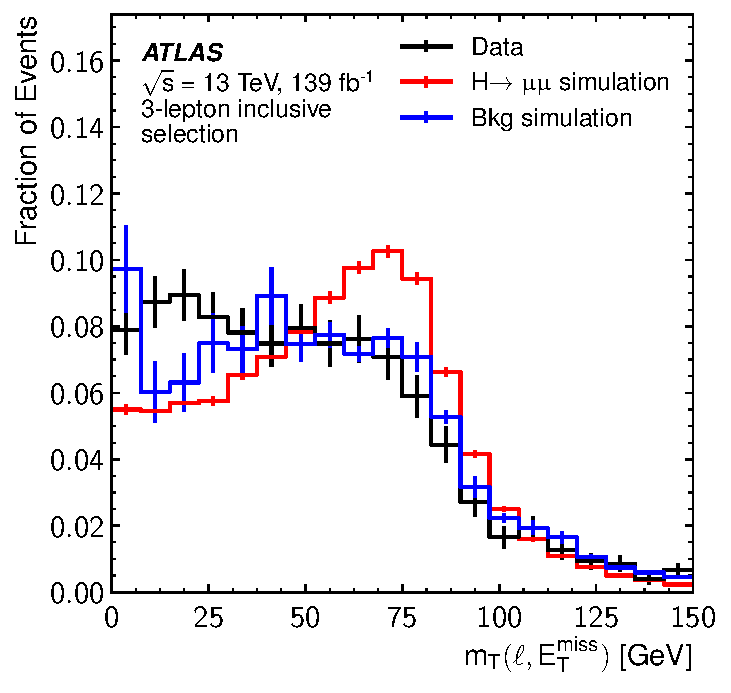
\includegraphics[width=0.35\textwidth]{figures/hmm/public/kine/kine-3lep-aux1_met_mt.pdf}}}
\subfloat[][]{{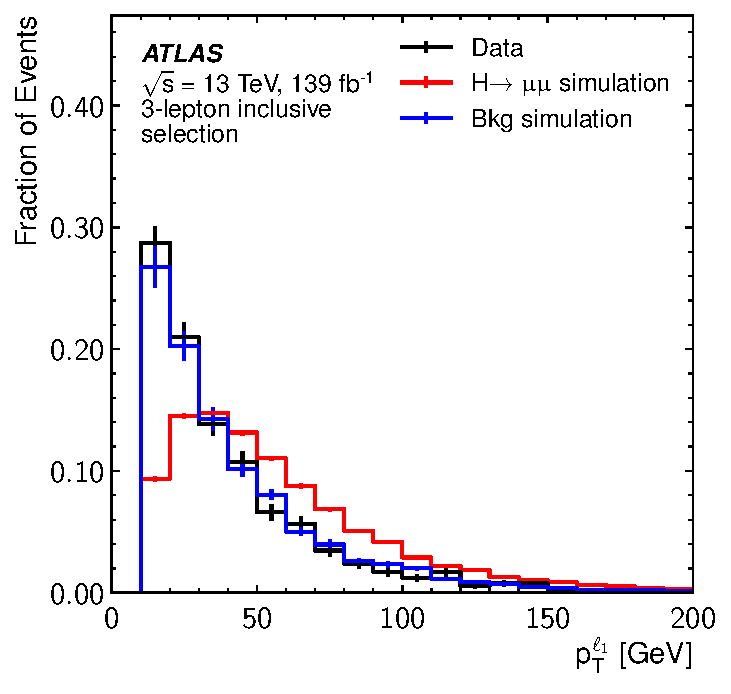
\includegraphics[width=0.35\textwidth]{figures/hmm/public/kine/kine-3lep-aux1_pt.pdf}}}
\subfloat[][]{{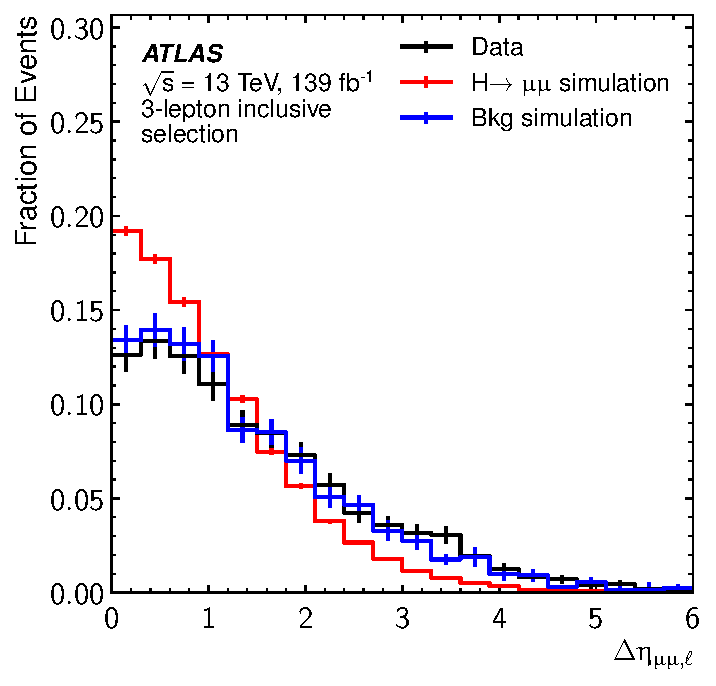
\includegraphics[width=0.35\textwidth]{figures/hmm/public/kine/kine-3lep-aux1_uu_delta_eta.pdf}}} \\
\subfloat[][]{{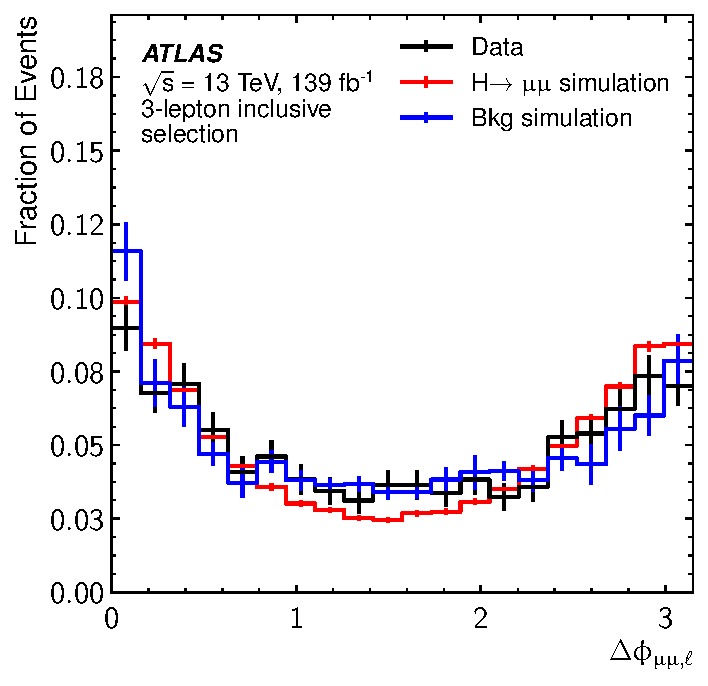
\includegraphics[width=0.35\textwidth]{figures/hmm/public/kine/kine-3lep-aux1_uu_delta_phi.pdf}}}
\subfloat[][]{{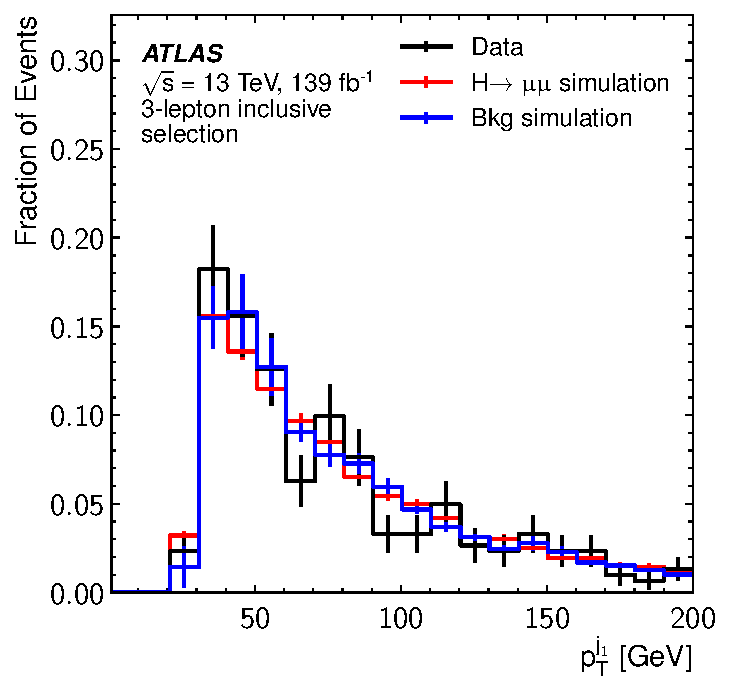
\includegraphics[width=0.35\textwidth]{figures/hmm/public/kine/kine-3lep-j1_pt.pdf}}}
\subfloat[][]{{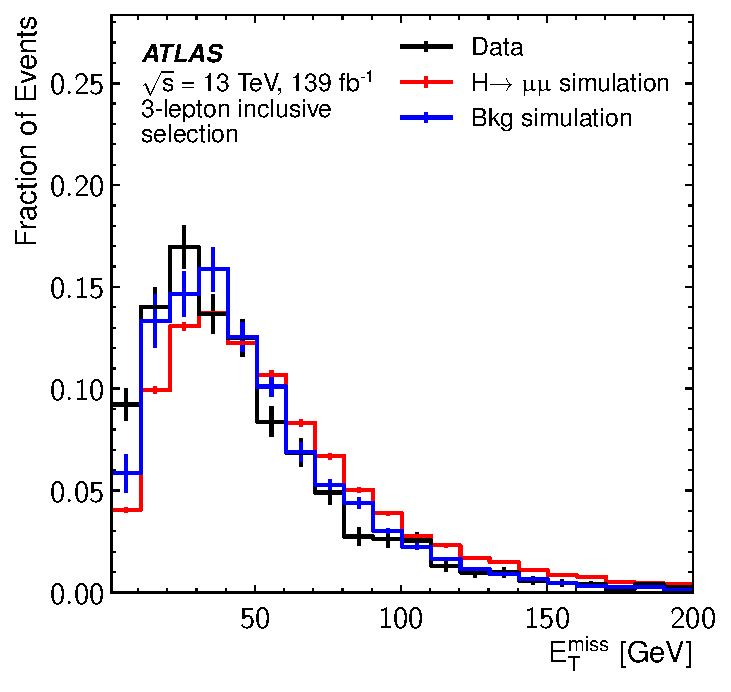
\includegraphics[width=0.35\textwidth]{figures/hmm/public/kine/kine-3lep-met_pt.pdf}}} \\
\subfloat[][]{{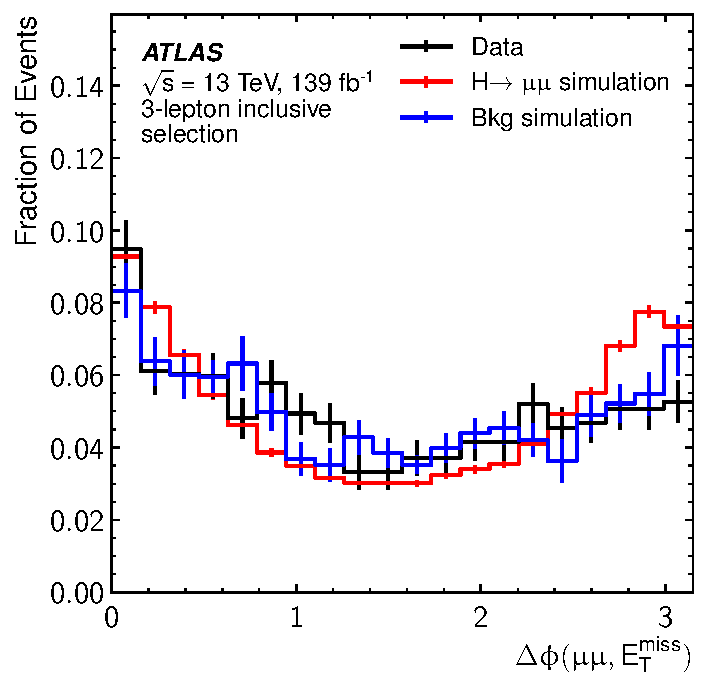
\includegraphics[width=0.35\textwidth]{figures/hmm/public/kine/kine-3lep-met_uu_delta_phi.pdf}}}
\subfloat[][]{{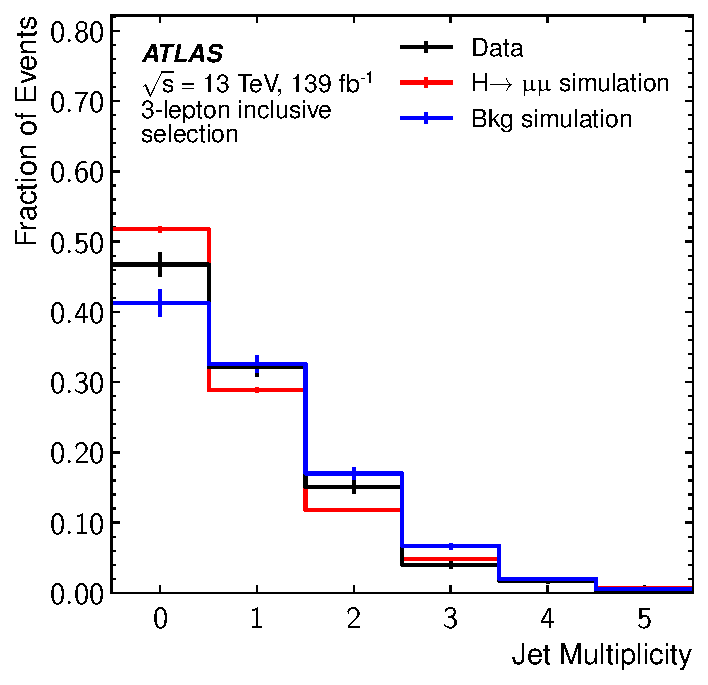
\includegraphics[width=0.35\textwidth]{figures/hmm/public/kine/kine-3lep-nJets.pdf}}}
\caption{Training variables provided as input for the for the 3-lepton classifier. The signal distribution shown in red is comprised of specifically the simulated WH signal dataset, while the background distribution contains all background shown in blue production modes. Data distributions are included in black. Each distribution is normalized, and the error bars on each histogram are statistical only. }
\label{fig:hmm3lepVars}
\end{figure}
\clearpage
}

\afterpage{
\begin{figure}[h!]
\captionsetup[subfigure]{position=b}
\centering
\subfloat[][]{{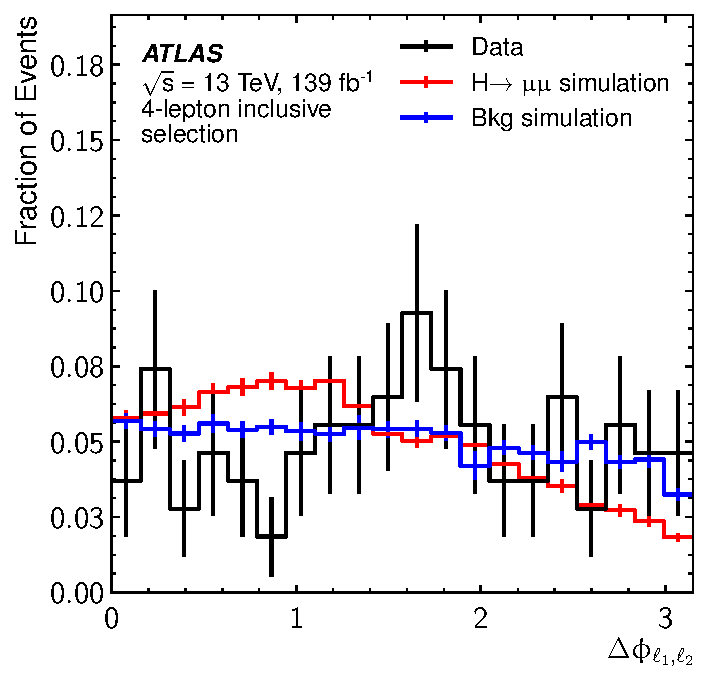
\includegraphics[width=0.35\textwidth]{figures/hmm/public/kine/kine-4lep-auxDilep_delta_phi.pdf}}}
\subfloat[][]{{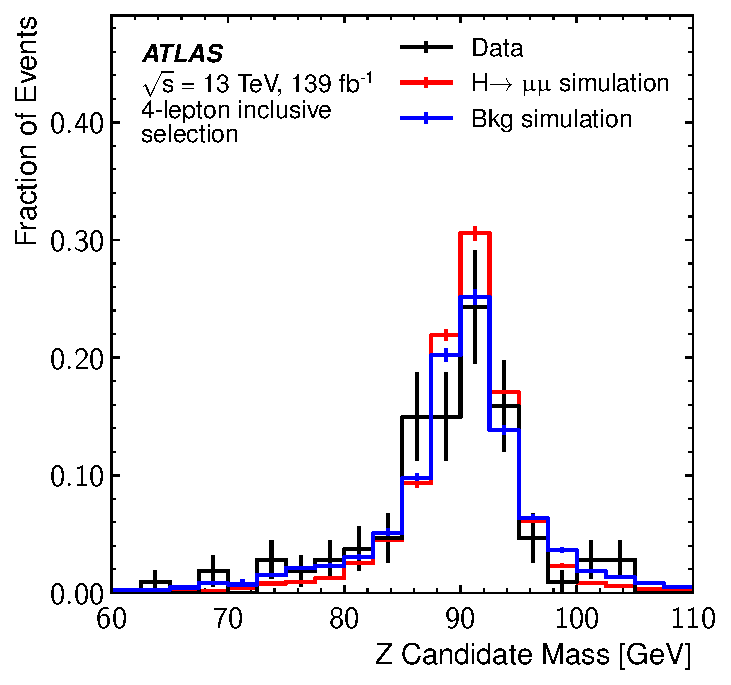
\includegraphics[width=0.35\textwidth]{figures/hmm/public/kine/kine-4lep-auxDilep_mass.pdf}}}
\subfloat[][]{{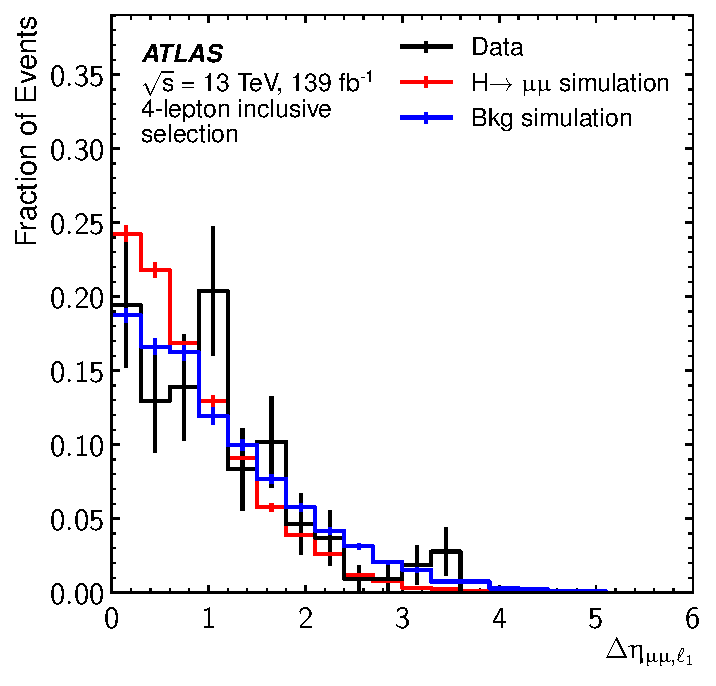
\includegraphics[width=0.35\textwidth]{figures/hmm/public/kine/kine-4lep-aux_uu_delta_eta.pdf}}} \\
\subfloat[][]{{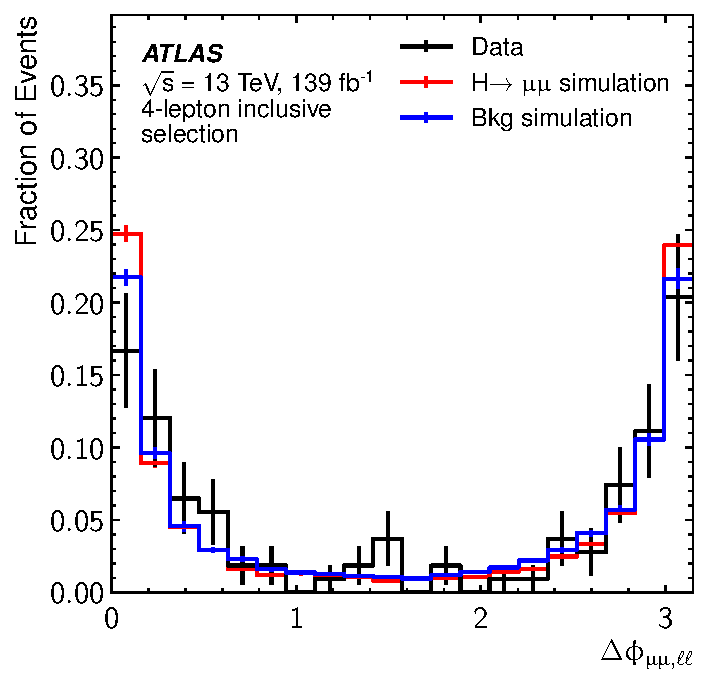
\includegraphics[width=0.35\textwidth]{figures/hmm/public/kine/kine-4lep-aux_uu_delta_phi.pdf}}}
\subfloat[][]{{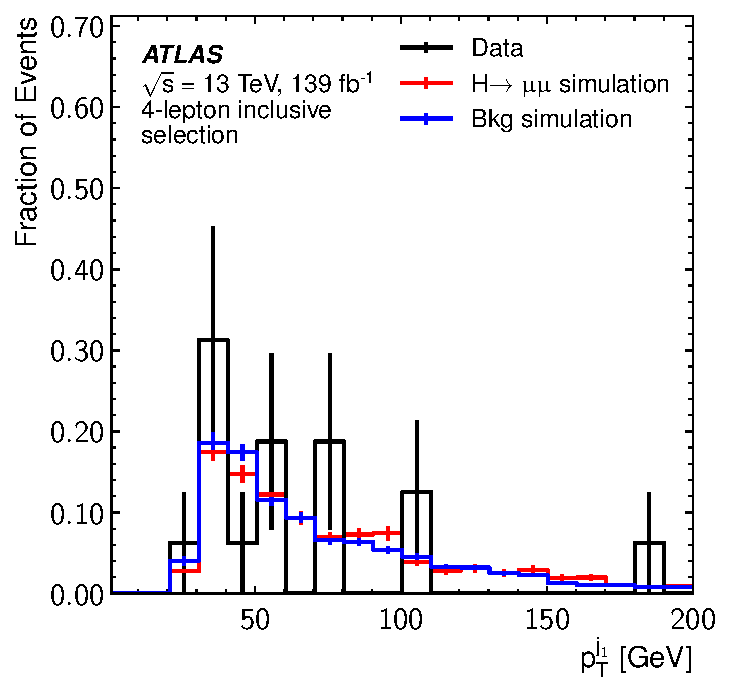
\includegraphics[width=0.35\textwidth]{figures/hmm/public/kine/kine-4lep-j1_pt.pdf}}}
\subfloat[][]{{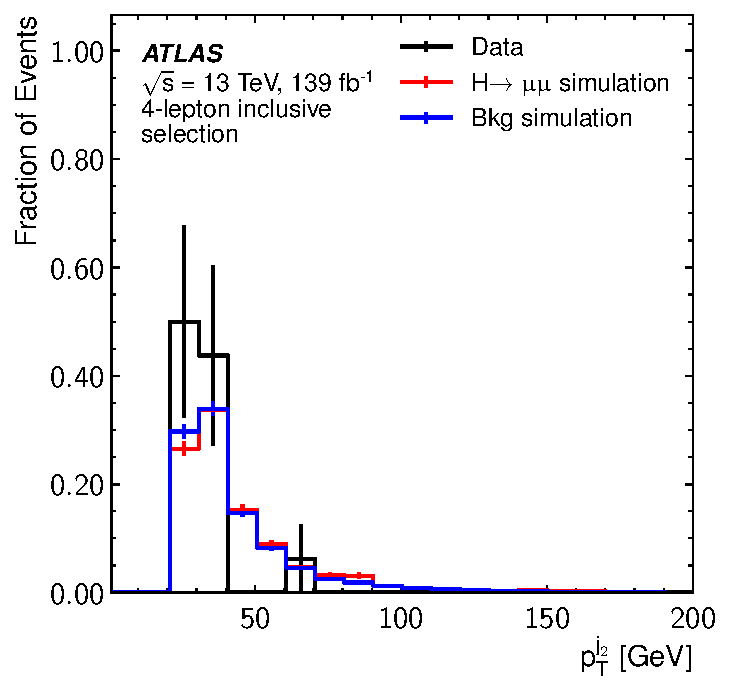
\includegraphics[width=0.35\textwidth]{figures/hmm/public/kine/kine-4lep-j2_pt.pdf}}} \\
\subfloat[][]{{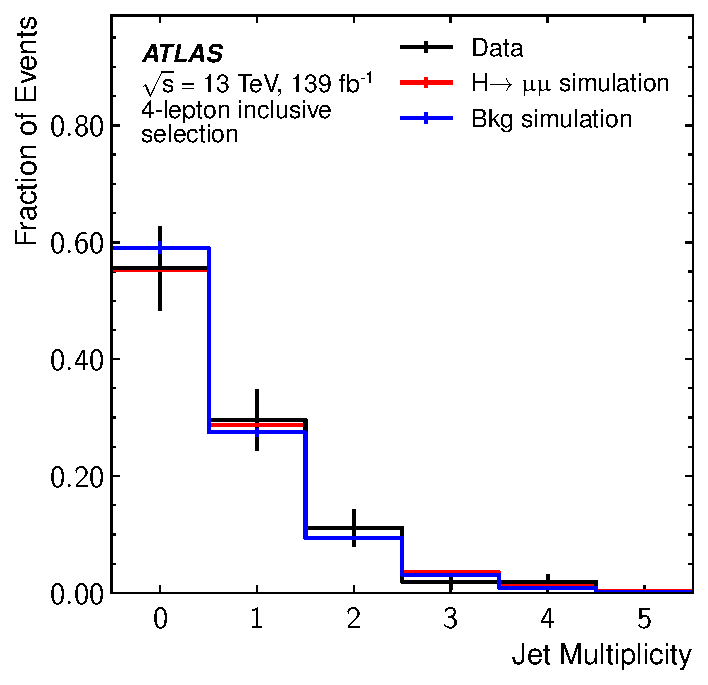
\includegraphics[width=0.35\textwidth]{figures/hmm/public/kine/kine-4lep-nJets.pdf}}}
\caption{Training variables provided as input for the for the 4-lepton classifier. The signal distribution shown in red is comprised of specifically the simulated WH signal dataset, while the background distribution contains all background shown in blue production modes. Data distributions are included in black. Each distribution is normalized, and the error bars on each histogram are statistical only. }
\label{fig:hmm4lepVars}
\end{figure}
\clearpage
}


%%%%%%%%%%%% Variable importance

% \begin{figure}[htpb]
%   \centering
%   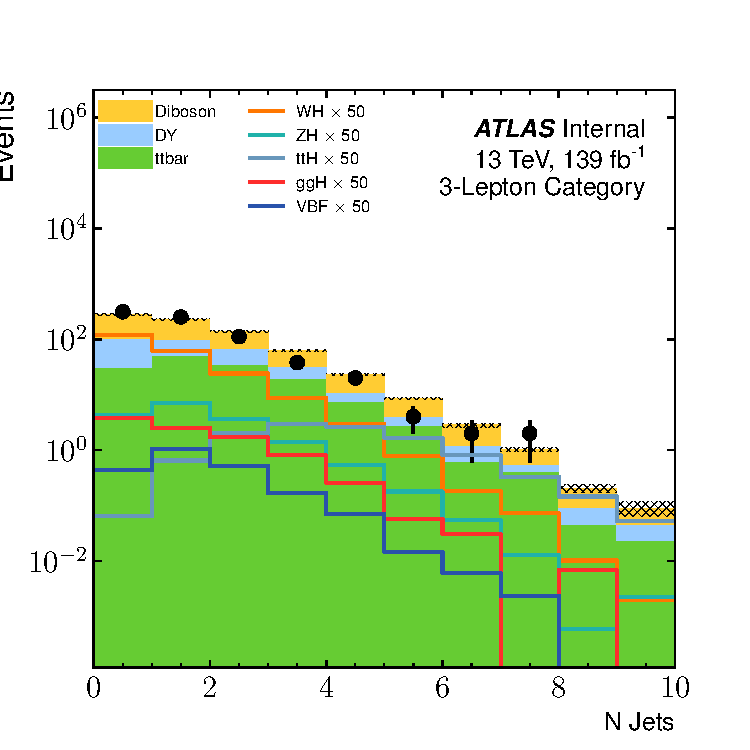
\includegraphics[height=0.48\textwidth]{figures/hmm/nJets/histo-3lep-nJets.pdf}
%   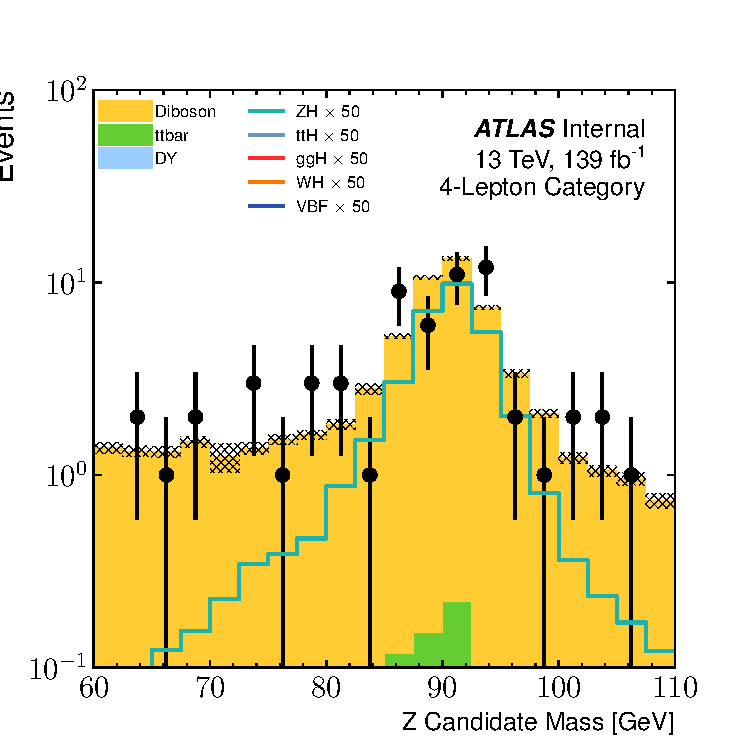
\includegraphics[height=0.48\textwidth]{figures/hmm/zCand/histo-4lep-auxDilep_mass.pdf}
%   \caption{Left: N Jets distribution for 3-lepton channel, right: Z candidate mass for 4-lepton channel. These are the highest ranked in feature importance for their category's respective BDT's.}
%     \label{fig:hmmImpVars}
% \end{figure}

The feature importance of the variables used in the training is shown in the plots of figure \ref{fig:hmmVarImport}.
In the 4-lepton case, the most important variable is the mass of the \Z candidate, which helps identify the signal.
In the 3-lepton case, the most important variable is the number of jets, which helps especially to separate out top quark backgrounds.

\begin{figure}[htpb]
  \centering
  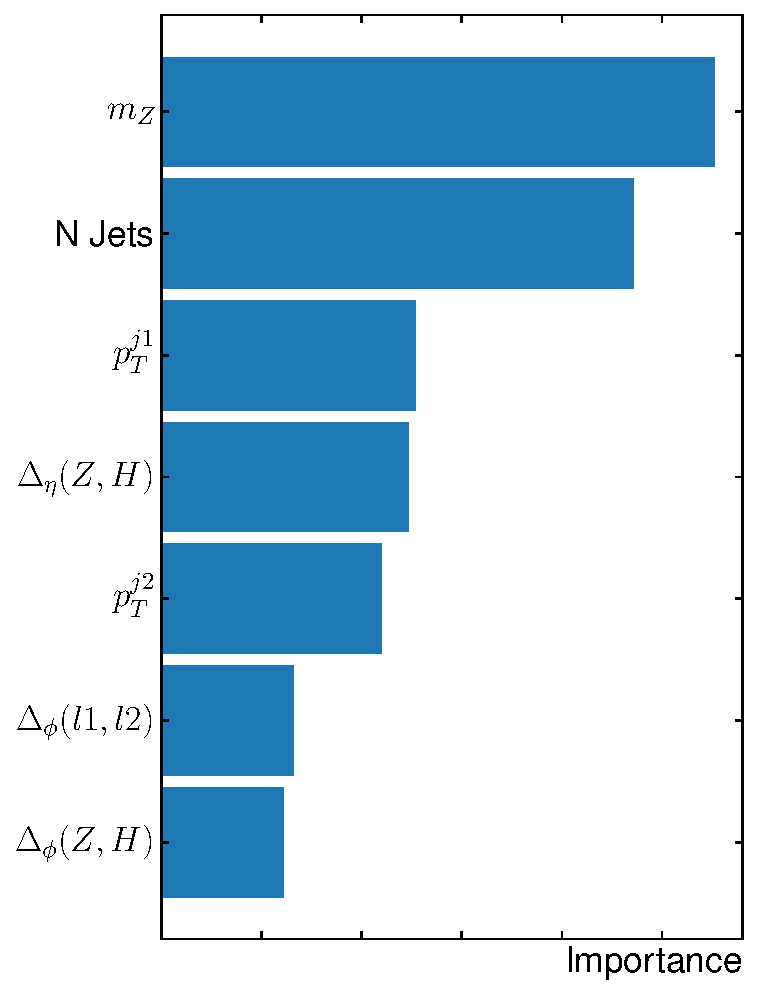
\includegraphics[height=8cm]{figures/hmm/bdtImportance/imp-4lep.pdf}
  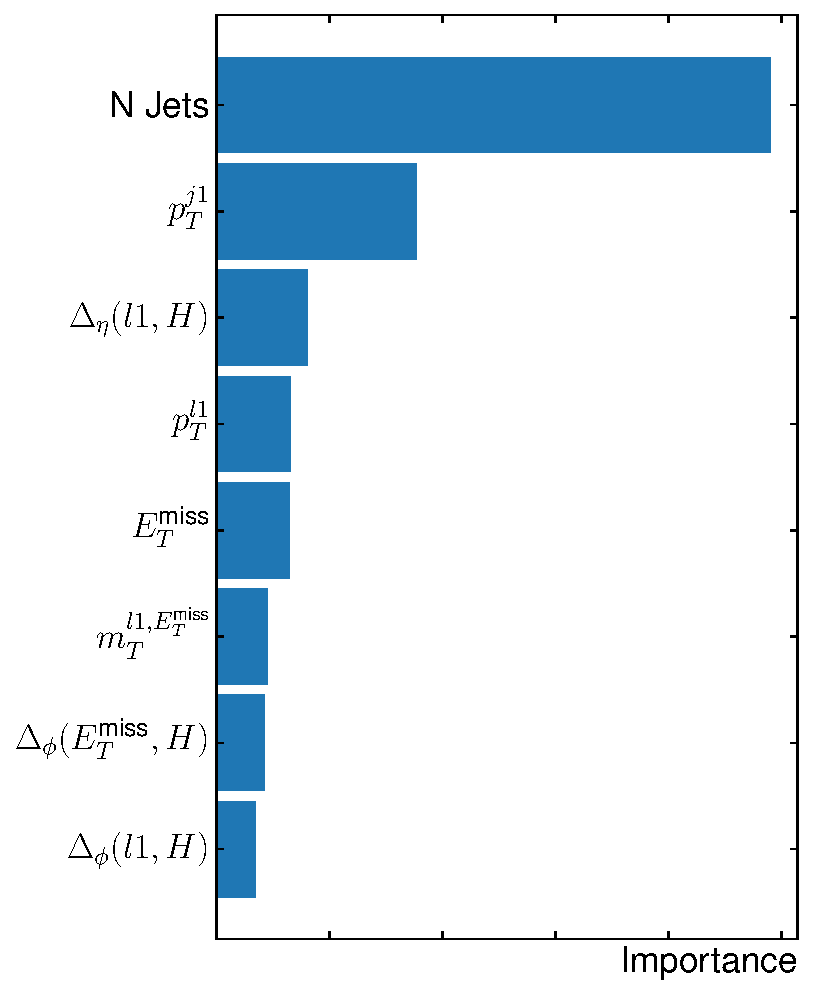
\includegraphics[height=8cm]{figures/hmm/bdtImportance/imp-3lep.pdf}
  \caption{The 4-lepton (left) and 3-lepton (right) variables shown with their respective feature importance, averaged over the five BDTs trained for each cross-validation permutation. The importance of a variable is defined relative to the other variables.}
    \label{fig:hmmVarImport}
\end{figure}

The performance of a BDT is measured using the validation scores of the receiver operator curve (ROC).
The ROC is a parametric function of the BDT discriminant, plotted as the rate of correct signal categorizations (true positive rate) compared to the rate of false categorization of background as signal (false positive rate).
This is plotted in Figure \ref{fig:hmmBdtRoc} for a number of discriminant thresholds that define signal versus background.
A figure of merit used to evaluate the ROC is area-under-curve (AUC).
These show comparable performance for the BDTs of both categories and the impact of the relatively limited statistics of the 4-lepton sample.
As a cross check, the ROC curve for the training set is plotted along with the validation set. The agreement between these, within statistical uncertainty, does not indicate clear over-training effects.
The signal and background samples shown in the ROC plots correspond to the same samples used for the training; only WH and ZH signals are used in the definition of the ROC.

\begin{figure}[htpb]
  \centering
  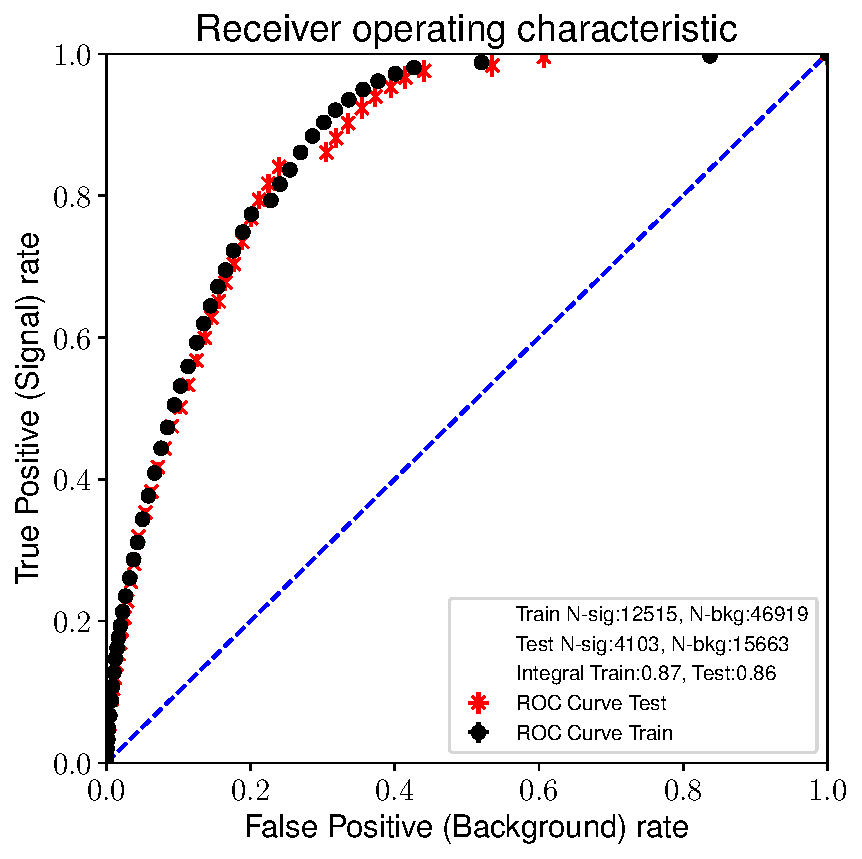
\includegraphics[width=0.48\textwidth]{figures/hmm/bdtHist/roc-4lep-ZH-AllBackground-0-depth2-nEst80tag-new-AllBackground.pdf}
  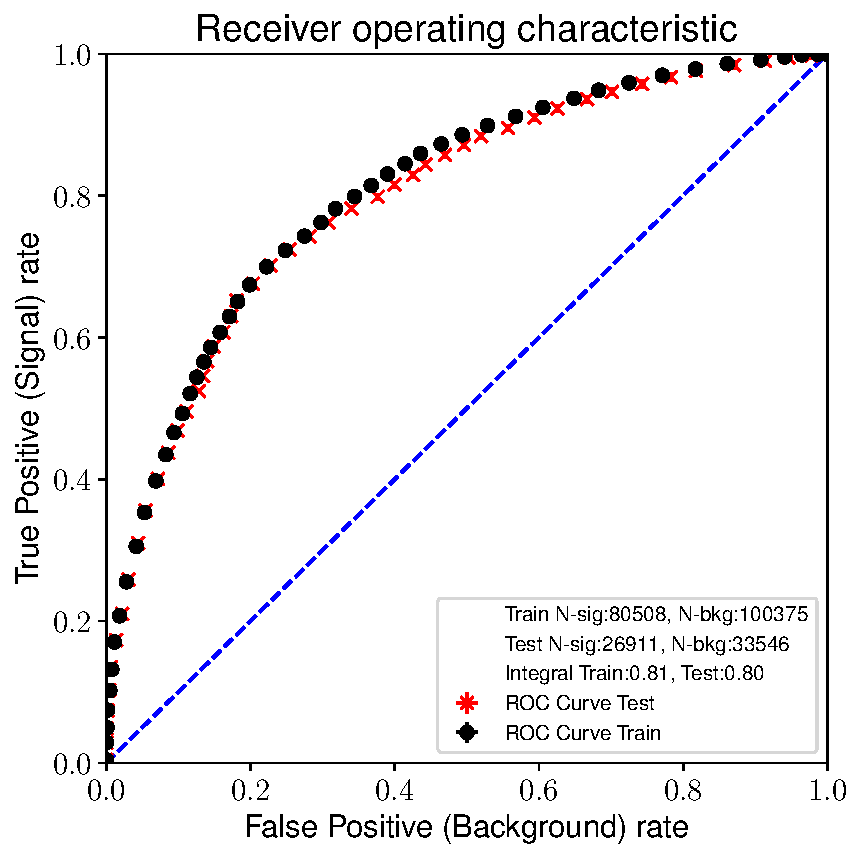
\includegraphics[width=0.48\textwidth]{figures/hmm/bdtHist/roc-3lep-WH-AllBackground-0-depth2-nEst50tag-new-AllBackground.pdf}
  \caption{4 lepton (left) and 3 lepton (right) ROC curves for representative BDT's. Shown in black is the curve for the training set, while red shows the curve for the validation set (labeled test set). Error bars are statistical uncertainties due to the size of the training and validation datasets. The AUC is labeled on each plot.}
    \label{fig:hmmBdtRoc}
\end{figure}

% Figure \ref{fig:hmmBdtScoreLin} shows distributions of the BDT discriminant for different categories of signal and background, scaled the samples cross-section and luminosity.
% The signal/background separation is more apparent in this plot than in those normalized to the physical expectation.


% \begin{figure}[htpb]
%   \centering
%   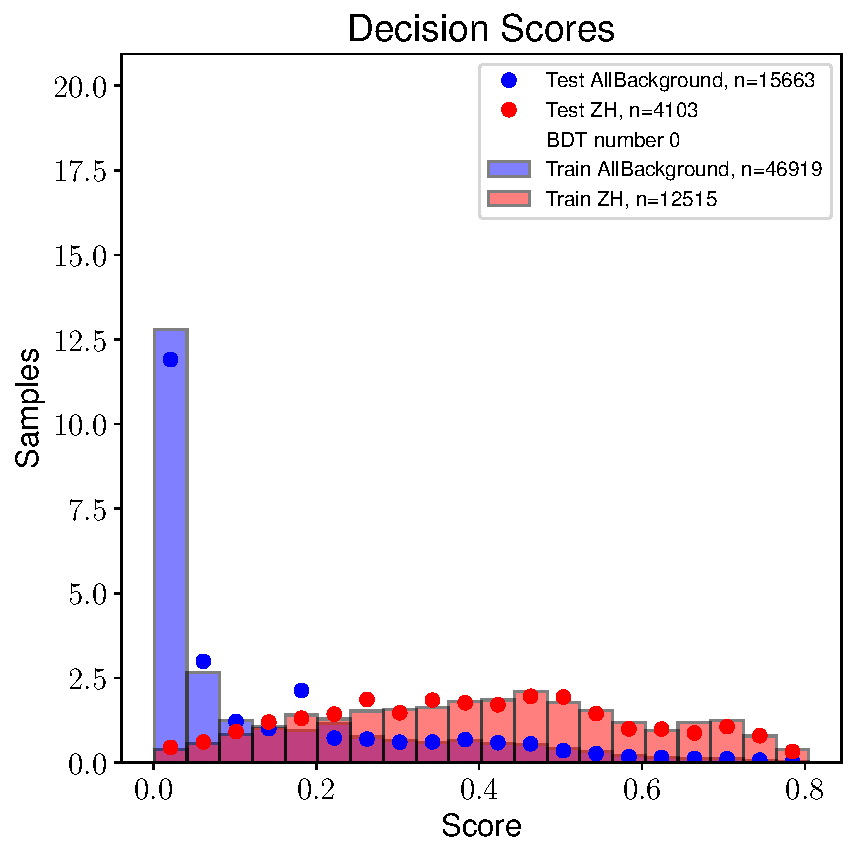
\includegraphics[width=0.48\textwidth]{figures/hmm/bdtHist/bar20-4lep-ZH-AllBackground-0-depth2-nEst80tag-new-AllBackground.pdf}
%   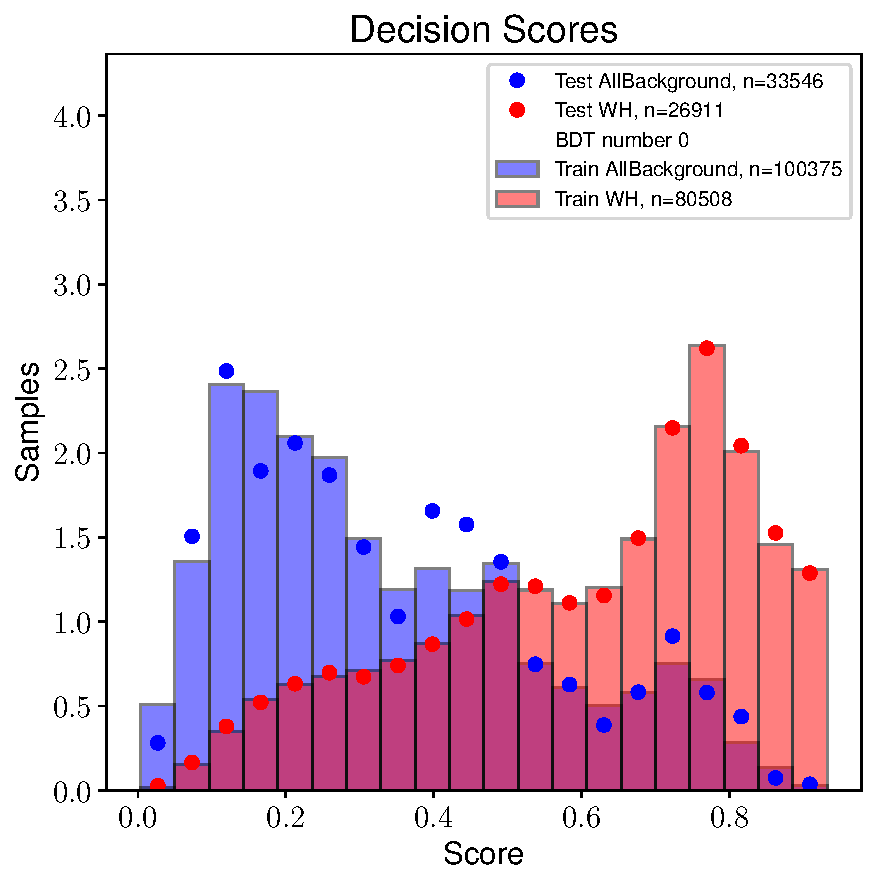
\includegraphics[width=0.48\textwidth]{figures/hmm/bdtHist/bar20-3lep-WH-AllBackground-0-depth2-nEst50tag-new-AllBackground.pdf}
%   \caption{4 lepton (left) and 3 lepton (right) distributions of the BDT discriminant, where the signal and background samples share a normalization. The signal distribution is that of the sample used for training, not the full signal MC sample.}
%     \label{fig:hmmBdtScoreLin}
% \end{figure}

Figure \ref{fig:hmmBdtScore} shows the BDT discriminant calculated in different categories and scaled by the samples cross-section and luminosity.
The signal and background composition is more apparent in these plots: primarily, the target signal production mechanism is separated from other signals.
The top backgrounds are particularly well separated owing in part to the high statistics available for these samples in the training sets.

% {\color{red} This paragraph section is slightly redundant. Merge into next section?}
% Exclusive categories are defined based on discriminant cuts that produce varying levels of signal purity.
% The category ``4-lepton high-purity'' is defined in the 4-lepton selection by requiring 4-lepton BDT score greater than 0.12. 
% Two categories are defined from the 3-lepton selection: ``3-lepton high-purity'' and ``3-lepton middle-purity''. 
% The former is selected by requiring 3-lepton BDT score greater than 0.7,
% and the latter is selected by requiring 3-lepton BDT score less than 0.7
% but greater than 0.1.
% The events failing VH categorization are still considered in the inclusive categories.
 
\begin{figure}[htpb]
  \centering
  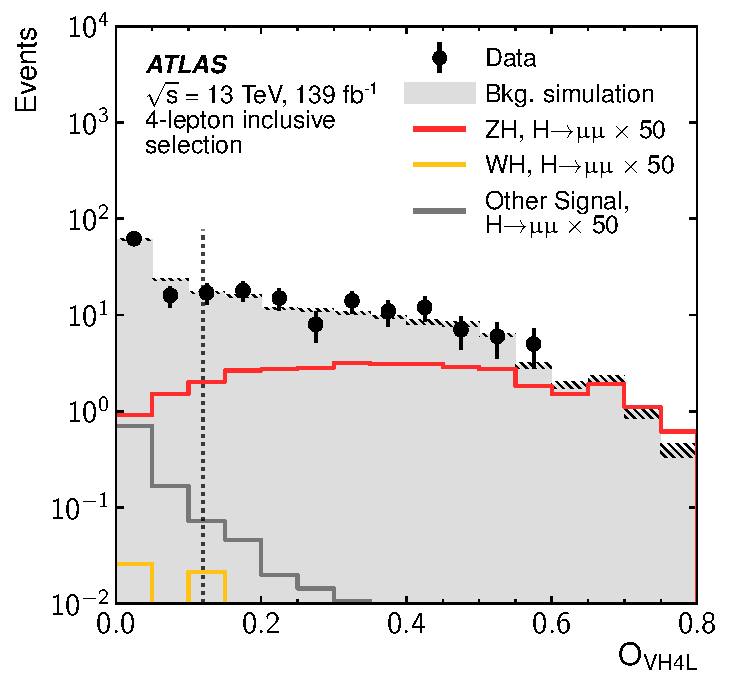
\includegraphics[width=0.48\textwidth]{figures/hmm/public/bdt/histo-4lep-bdtScore.pdf}
  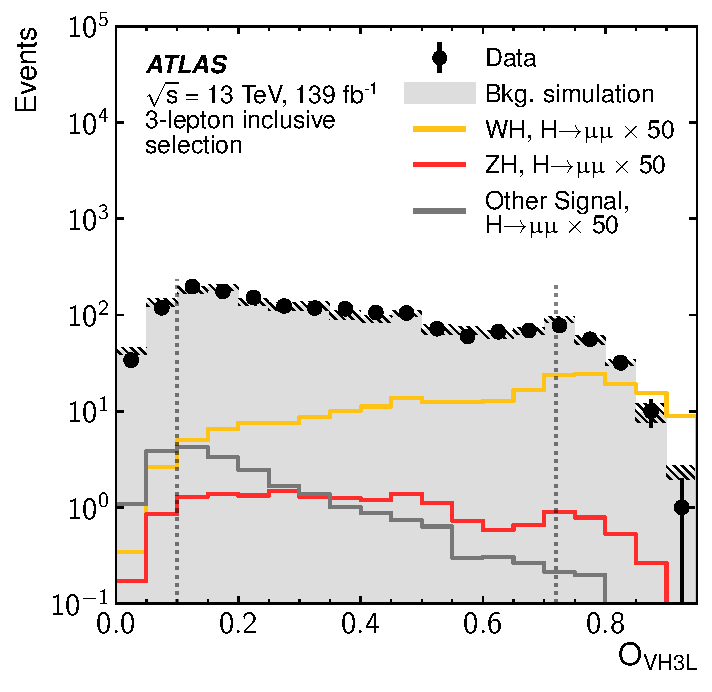
\includegraphics[width=0.48\textwidth]{figures/hmm/public/bdt/histo-3lep-bdtScore.pdf}
  \caption{4-lepton (left) and 3-lepton (right) distributions of the BDT discriminant, using the final test scores. The simulated background is shown in shaded grey, while the signal distributions are drawn as lines in red for ZH and orange for WH. The remaining non-VH production mechanisms (ggF, VBF, and ttH) are combined and plotted as a dark grey line. All the signal histograms have been scaled by a factor of 50 to enhance visibility.\\
  It is observed that the score separates the signal to the left and background to the right. Of similar importance is that it specifically isolates the VH signal of interest and not the other signal productions. For 4-lepton this is the ZH signal and for 3-lepton this is the WH signal. Vertical dotted lines indicate the values that delineate which events belong in which final categories. The full dataset is included as well, which is used to fix the normalization of the background. \\
  The 3-lepton discriminant separates signal from background to a higher degree than does the 4-lepton discriminant. This is due in part to the stricter 4-lepton event selection, which can remove many more ``easily'' separable background events. The remaining events are more similar, topologically, to the ZH signal.}
    \label{fig:hmmBdtScore}
\end{figure}

\subsection{Categorization}

The event selection results in two selections: 4-lepton and 3-lepton.
Next, using the BDT discriminant scores, these selections are further divided into \emph{exclusive} categories based on the relative purity of the signal.
The 4-lepton category is divided once into low-purity and high-purity categories.
The 3-lepton category, since the event multiplicity is higher, is divided into low-, medium-, and high-purity categories.

Each event belongs to both a validation dataset and a testing dataset, each of which has an associated discriminant score.
The validation scores are considered when selecting the score thresholds delineating categories.
The testing scores are used for the final hypothesis test and limit setting.
An optimization scan over various thresholds of the expected significance is performed.
The thresholds are selected in order to produce the highest expected significance, based on the validation scores.
These thresholds are specified in Table \ref{tab:hmmBdtCuts}.

\begin{table}[htp]
\begin{center}
\begin{tabular}{l l l l}
\toprule
Category & Discriminant \\
\midrule
4-Lepton High-purity & $O\ge0.12$ \\
4-Lepton Low-purity & $O<0.12$ \\
3-Lepton High-purity & $O\ge0.72$ \\
3-Lepton Middle-purity & $0.10\ge O<0.72$ \\
3-Lepton Low-purity & $O<0.10$ \\
\bottomrule
\end{tabular}
\caption{Category definitions based on the ranges of the discriminant value $O$. The output of the BDT is scaled such that $O\in[0,1]$.}
\label{tab:hmmBdtCuts}
\end{center}
\end{table}

To pick the score thresholds using the testing set, and then perform a hypothesis test in categories defined by that threshold would lead to a misleading signal and background expectation in those categories.
The choice of threshold would be biased to the statistical fluctuations in the test dataset.
This results in categories biased to contain more simulated signal events and fewer simulated background events than would be expected in the data.
Since the analysis of the data includes the signal model based on simulation, such a method is unacceptable.

\begin{figure}[htpb]
  \centering
  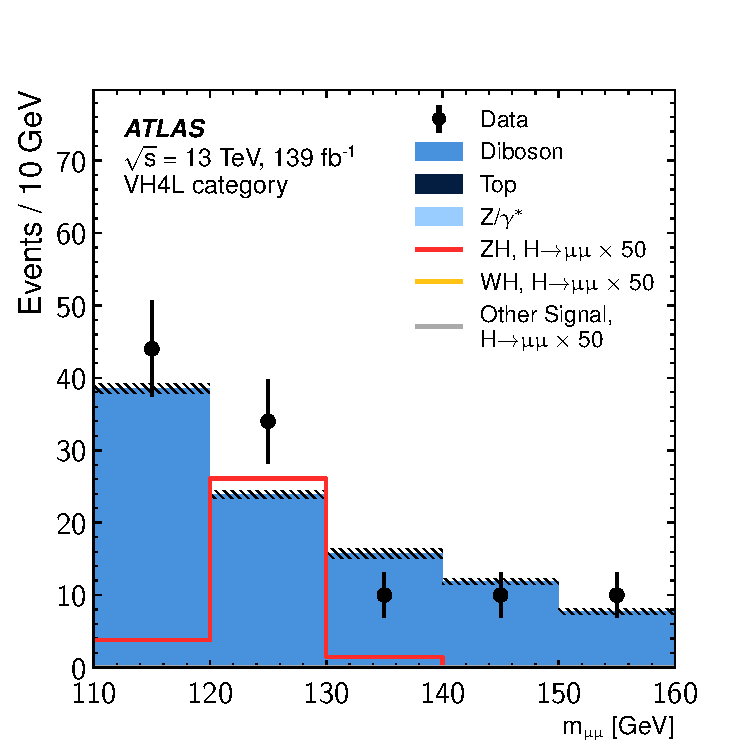
\includegraphics[width=0.45\textwidth]{figures/hmm/public/postCut/histo-4lep0-muu.pdf} \\
  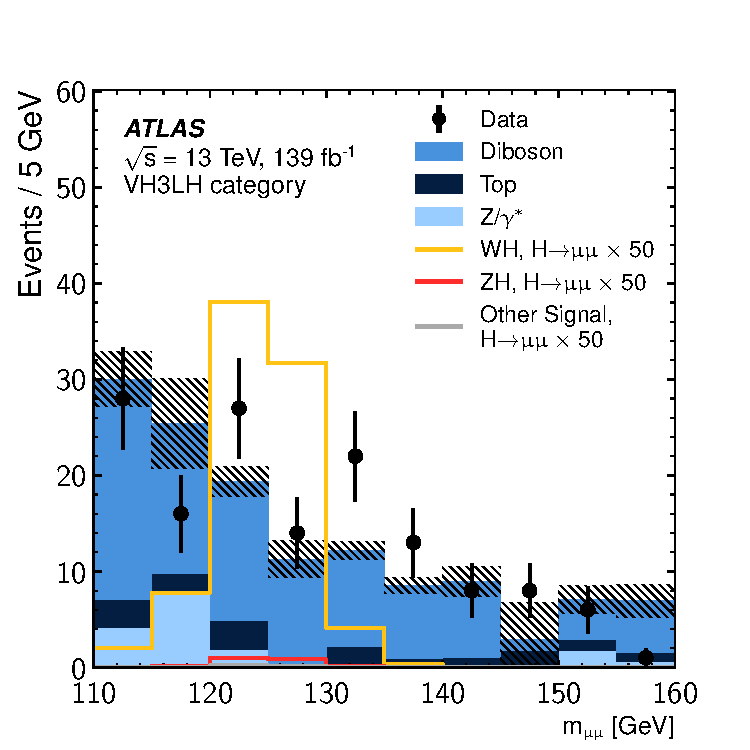
\includegraphics[width=0.45\textwidth]{figures/hmm/public/postCut/histo-3lep0-muu.pdf} 
  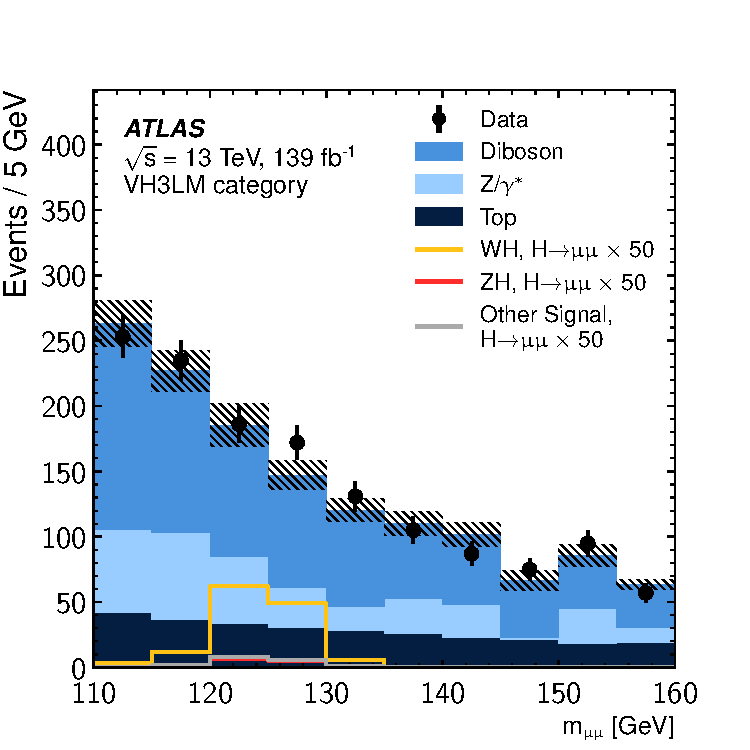
\includegraphics[width=0.45\textwidth]{figures/hmm/public/postCut/histo-3lep1-muu.pdf} 
  \caption{Distributions of \muu in the 4-lepton (top) and 3-lepton (bottom) categories after a cut on the BDT discriminant.}
    \label{fig:hmmPostcutMassHists}
\end{figure}
\clearpage

The high and middle-purity categories are considered for further analysis.
The low-purity events, containing few expected signal events, are only analyzed in the inclusive categories defined prior to BDT cut.
The distributions of \muu are shown in Figures \ref{fig:hmmPrecutMassHists} and \ref{fig:hmmPostcutMassHists}.
The former shows the inclusive distribution before further categorization with the BDT discriminant.
The latter shows the distributions in the categories defined in Table \ref{tab:hmmBdtCuts}.
The motivation to use the discriminant becomes apparent in these plots when compared to Figure \ref{fig:hmmPrecutMassHists}.
In both the 4-lepton and 3-lepton high-purity categories, Drell-Yan production has been virtually removed.
The background remaining is primarily from diboson sources.
The signal selection purity is also evident in the high-purity categories: the categories select homogeneous ZH or WH depending on their target.

